% Gemini theme
% See: https://rev.cs.uchicago.edu/k4rtik/gemini-uccs
% A fork of https://github.com/anishathalye/gemini

\documentclass[final]{beamer}

% ====================
% Packages
% ====================
\usepackage{amsfonts}
\usepackage[T1]{fontenc}
\usepackage{lmodern}
\usepackage[size=custom,width=120,height=72,scale=1.0]{beamerposter}
\geometry{paperwidth=42in,paperheight=32.5in}
\usetheme{gemini}
\usecolortheme{ucf}
\usepackage{graphicx}
\usepackage{booktabs}
\usepackage{tikz}
\usepackage{pgfplots}
\usepackage{natbib}
\pgfplotsset{compat=1.17}

% ====================
% Lengths
% ====================

% If you have N columns, choose \sepwidth and \colwidth such that
% (N+1)*\sepwidth + N*\colwidth = \paperwidth
\newlength{\sepwidth}
\newlength{\colwidth}
\setlength{\sepwidth}{0.025\paperwidth}
\setlength{\colwidth}{0.3\paperwidth}

\newcommand{\separatorcolumn}{\begin{column}{\sepwidth}\end{column}}

% ====================
% Title
% ====================

\title{Application of Random Forest to classify EEG data of mTBI patients and control adults obtained during a Visuospatial Working Memory Task}

\author{Cruz, W.,\inst{1} Cavanagh, J.F.,\inst{2} \and Lin, C.Y.\inst{1}}

\institute[shortinst]{\inst{1} \textit{National ChengKung University, NCKU} \samelineand \inst{2} University of New Mexico, UNM}

% ====================
% Footer (optional)
% ====================

\footercontent{
  \href{https://github.com/billytaipei101}{https://github.com/billytaipei101} \hfill
  Vision Sciences Society Symposia 2022, Florida FL\hfill
  \href{mailto:wi.cruzm@gmail.com}{wi.cruzm@gmail.com}}
% (can be left out to remove footer)

% ====================
% Logo (optional)
% ====================

% use this to include logos on the left and/or right side of the header:
% \logoright{\includegraphics[height=7cm]{logo1.pdf}}
% \logoleft{\includegraphics[height=7cm]{logo2.pdf}}

% ====================
% Body
% ====================

\begin{document}
\addtobeamertemplate{headline}{}
{
    \begin{tikzpicture}[remember picture,overlay]
      \node [anchor=north west, inner sep=3cm] at ([xshift=2cm,yshift=-0.8cm]current page.north west)
      {
\includegraphics[height=7.5cm]{logos/z_logo.png}}; % also try shield-white.eps
      \node [anchor=north east, inner sep=3cm] at ([xshift=0cm,yshift=-1.1cm]current page.north east)
      {
\includegraphics[height=6.5cm]{logos/University_of_New_Mexico.png}};
    \end{tikzpicture}
}

\begin{frame}[t]
\begin{columns}[t]
\separatorcolumn

\begin{column}{\colwidth}

  \begin{block}{Introduction}

    The combination of electroencephalographic (EEG) recording and cognitive experimental tasks provides an excellent tool for studying human neural dynamics. EEG provides high temporal resolution time series data sampled across multiple scalp locations that produces large amounts of data, and some of these datasets are freely available in repositories on the internet (Fig. 1). 

    \begin{figure}
      \centering
      
\includegraphics[width=25cm]{img/bids2.png} 
      \caption{Open-science neuroinformatics database repository.}
    \end{figure}

    Most of the time the analysis of such data requires the implementation of many signal extraction methods that are further used to characterize the psycho physiological phenomena being studied. Sometimes the large amount of data collected for one experiment is not fully used because most of the researchers prefer to take a confirmatory and deductive approach, thus focusing their attention in a rather narrow number of features but unintentially overlooking other important latent  features.
    The utility of the random forest algorithm was investigated as a computational framework for extracting the most relevant features from an EEG data set obtained from an online repository (RRID: ds003523) with data of mild Traumatic Brain Injury (mTBI) patients and Healthy Controls (HC) during a Visuospatial Working Memory (VSWM) Task . 

    Random forest is a supervised ML method mostly used for classification purposes; the algorithm generates a set number of decision trees, each of which is made based on different subsets of data extracted from the training set. These subsets are selected following a random sampling approach; this iterative process  and the number of decision trees computed are further used to reach a classification consensus, and the most common output is selected as the most relevant model which is usually the one that contains the most relevant features for the purpose of classifying the cases or instances being considered. Therefore it is possible to use EEG signal recording along with this classification framework to characterize the neural dynamics and predict both, performance and diagnosis.

  \end{block}

  \begin{block}{Advantages of Analyzing EEG data with ML algorithms}

  Machine Learning techniques include different computational frameworks that are capable of mining large datasets, some advantages of using these frameworks when analyzing EEG datasets are:

    \begin{itemize}
      \item \textbf{Identify} relevant questions concerning EEG data.
      \item \textbf{Discover} new knowledge through pattern recognition and mathematical modeling.
      \item \textbf{Applicability} in both medical and social sciences.
      \item \textbf{Predict} the performance in a task.
      \item \textbf{Diagnose} patients based on their neural activity patterns.
    \end{itemize}
  \end{block}

\end{column}

\separatorcolumn

\begin{column}{\colwidth}

  \begin{block}{Methods}

  The data used was obtained from an OpenNeuro repository but the subjects that conformed the final groups for the present analysis, mild Traumatic Brain Injury patients (mTBI, \textit{n = }27) and Healthy Controls (HC, \textit{n =}27), were matched using demographic variables and their score in a Visuospatial Working Memory (VSWM) task, thus ensuring that both groups did not differ significantly by age (\textit{p =} 0.67), sex (\textit{p =} 0.58), nor by hit ratio (\textit{p= }0.97). The EEG epoched signals covering three memory phases (i.e. Baseline, Encoding, Retention) were analyzed to extract 5 frequency components from each of the 63 scalp sites. The EEG data was labelled by group and separated as either correct or incorrect for classification purposes.
    
  \end{block}

  \begin{block}{Visuospatial Working Memory (VSWM) task}

In the VSMW task, participants had to perform a yes-no recognition task (see Figure 2) and were asked to respond whether a location defined by a square containing a question mark (i.e. probe) had been occupied by a red dot in the preceding visual array. Participants were told to ignore the yellow dots. Altogether there were three conditions, either showing three targets or three red dots (\textit{Condition 3}), showing three targets and two distractors (\textit{Condition 3 + 2}), or showing 5 targets (\textit{Condition 5})

    \begin{figure}
      \centering
     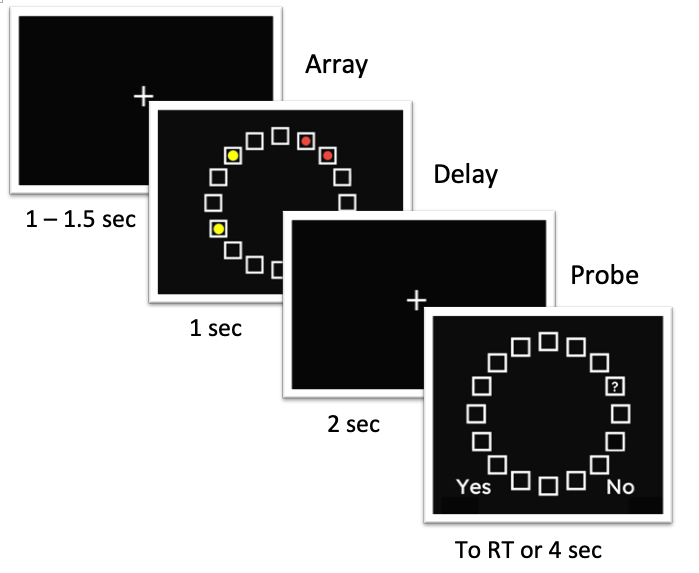
\includegraphics[width=24cm]{img/VSWM_task.png} 
      \caption{Visuospatial Working Memory (VSWM) task.}
    \end{figure}

  \end{block}

  \begin{block}{EEG data}
    
    EEG activity was recording using a 64 channel cap and the electrodes were located according to the 10-20 system. Additional electrodes were placed above and below the right orbit (VEOG) while simultaneously monitoring EKG activity. Continuous EEG was monitored and reference to the \textit{Fz} channel and acquired at a 1000 Hz sampling rate. The VSWM task was administered using MATLAB. Total EEG set up time was in average 30 minutes, and the VSWM task included a practice block and an experimental block with 150 trials.

    After the EEG signals were fully collected, the data of each subject was first loaded into EEGLab \citep{delorme2004eeglab}, then the EKG and VEOG were removed leaving only the channels that recorded brain activity. Following each subject's data was decomposed by ICA using the picard algorithm and the artifact components were removed with the SASICA module

    \begin{itemize}
      \item \textbf{Sed consequat} id ante vel efficitur. Praesent congue massa
        sed est scelerisque, elementum mollis augue iaculis.
        \begin{itemize}
          \item In sed est finibus, vulputate
            nunc gravida, pulvinar lorem. In maximus nunc dolor, sed auctor eros
            porttitor quis.
          \item Fusce ornare dignissim nisi. Nam sit amet risus vel lacus
            tempor tincidunt eu a arcu.
          \item Donec rhoncus vestibulum erat, quis aliquam leo
            gravida egestas.
        \end{itemize}
      \item \textbf{Sed luctus, elit sit amet} dictum maximus, diam dolor
        faucibus purus, sed lobortis justo erat id turpis.
      \item \textbf{Pellentesque facilisis dolor in leo} bibendum congue.
        Maecenas congue finibus justo, vitae eleifend urna facilisis at.
    \end{itemize}
    
    Nulla eget sem quam. Ut aliquam volutpat nisi vestibulum convallis. Nunc a
    lectus et eros facilisis hendrerit eu non urna. Interdum et malesuada fames
    ac ante \textit{ipsum primis} in faucibus. Etiam sit amet velit eget sem
    euismod tristique. Praesent enim erat, porta vel mattis sed, pharetra sed
    ipsum. Morbi commodo condimentum massa, \textit{tempus venenatis} massa
    hendrerit quis. Maecenas sed porta est. Praesent mollis interdum lectus,
    sit amet sollicitudin risus tincidunt non.
  \end{block}

\end{column}

\separatorcolumn

\begin{column}{\colwidth}

  \begin{block}{A block containing some math}

    Nullam non est elit. In eu ornare justo. Maecenas porttitor sodales lacus,
    ut cursus augue sodales ac.

    $$
    \int_{-\infty}^{\infty} e^{-x^2}\,dx = \sqrt{\pi}
    $$

    Interdum et malesuada fames $\{1, 4, 9, \ldots\}$ ac ante ipsum primis in
    faucibus. Cras eleifend dolor eu nulla suscipit suscipit. Sed lobortis non
    felis id vulputate.

    \heading{A heading inside a block}

    Praesent consectetur mi $x^2 + y^2$ metus, nec vestibulum justo viverra
    nec. Proin eget nulla pretium, egestas magna aliquam, mollis neque. Vivamus
    dictum $\mathbf{u}^\intercal\mathbf{v}$ sagittis odio, vel porta erat
    congue sed. Maecenas ut dolor quis arcu auctor porttitor.

    \heading{Another heading inside a block}

    Sed augue erat, scelerisque a purus ultricies, placerat porttitor neque.
    Donec $P(y \mid x)$ fermentum consectetur $\nabla_x P(y \mid x)$ sapien
    sagittis egestas. Duis eget leo euismod nunc viverra imperdiet nec id
    justo.

  \end{block}

  \begin{block}{Nullam vel erat at velit convallis laoreet}

    Class aptent taciti sociosqu ad litora torquent per conubia nostra, per
    inceptos himenaeos. Phasellus libero enim, gravida sed erat sit amet,
    scelerisque congue diam. Fusce dapibus dui ut augue pulvinar iaculis.

    \begin{table}
      \centering
      \begin{tabular}{l r r c}
        \toprule
        \textbf{First column} & \textbf{Second column} & \textbf{Third column} & \textbf{Fourth} \\
        \midrule
        Foo & 13.37 & 384,394 & $\alpha$ \\
        Bar & 2.17 & 1,392 & $\beta$ \\
        Baz & 3.14 & 83,742 & $\delta$ \\
        Qux & 7.59 & 974 & $\gamma$ \\
        \bottomrule
      \end{tabular}
      \caption{A table caption.}
    \end{table}

    Donec quis posuere ligula. Nunc feugiat elit a mi malesuada consequat. Sed
    imperdiet augue ac nibh aliquet tristique. Aenean eu tortor vulputate,
    eleifend lorem in, dictum urna. Proin auctor ante in augue tincidunt
    tempor. Proin pellentesque vulputate odio, ac gravida nulla posuere
    efficitur. Aenean at velit vel dolor blandit molestie. Mauris laoreet
    commodo quam, non luctus nibh ullamcorper in. Class aptent taciti sociosqu
    ad litora torquent per conubia nostra, per inceptos himenaeos.

    Nulla varius finibus volutpat. Mauris molestie lorem tincidunt, iaculis
    libero at, gravida ante. Phasellus at felis eu neque suscipit suscipit.
    Integer ullamcorper, dui nec pretium ornare, urna dolor consequat libero,
    in feugiat elit lorem euismod lacus. Pellentesque sit amet dolor mollis,
    auctor urna non, tempus sem.

  \end{block}



  \begin{block}{References}

    \nocite{*}
    \footnotesize{\bibliographystyle{apalike}\bibliography{r-references}}

  \end{block}

\end{column}

\separatorcolumn
\end{columns}
\end{frame}

\end{document}
